\documentclass{article}
\usepackage[utf8]{inputenc}
\usepackage[english]{babel}
\usepackage[font=small,labelfont=bf]{caption}
\usepackage{geometry}
\usepackage{natbib}
\usepackage{pxfonts}
\usepackage{graphicx}
\usepackage{newfloat}
\usepackage{setspace}
\usepackage{hyperref}
\usepackage{placeins}


\newcommand{\methodsdemo}{1}
\newcommand{\topicprops}{2}
\newcommand{\listlearning}{3}
\newcommand{\precisiondistinctiveness}{4}
\newcommand{\precisiondistinctivenessdetail}{5}
\newcommand{\trajectories}{6}
\newcommand{\wordles}{7}
\newcommand{\brains}{8}

\bibliographystyle{apa}

\begin{document}
\renewcommand{\figurename}{Supplementary Figure}
\setcounter{figure}{3}
\setcounter{page}{1}
\makeatletter

\begin{figure}[tp]
\centering
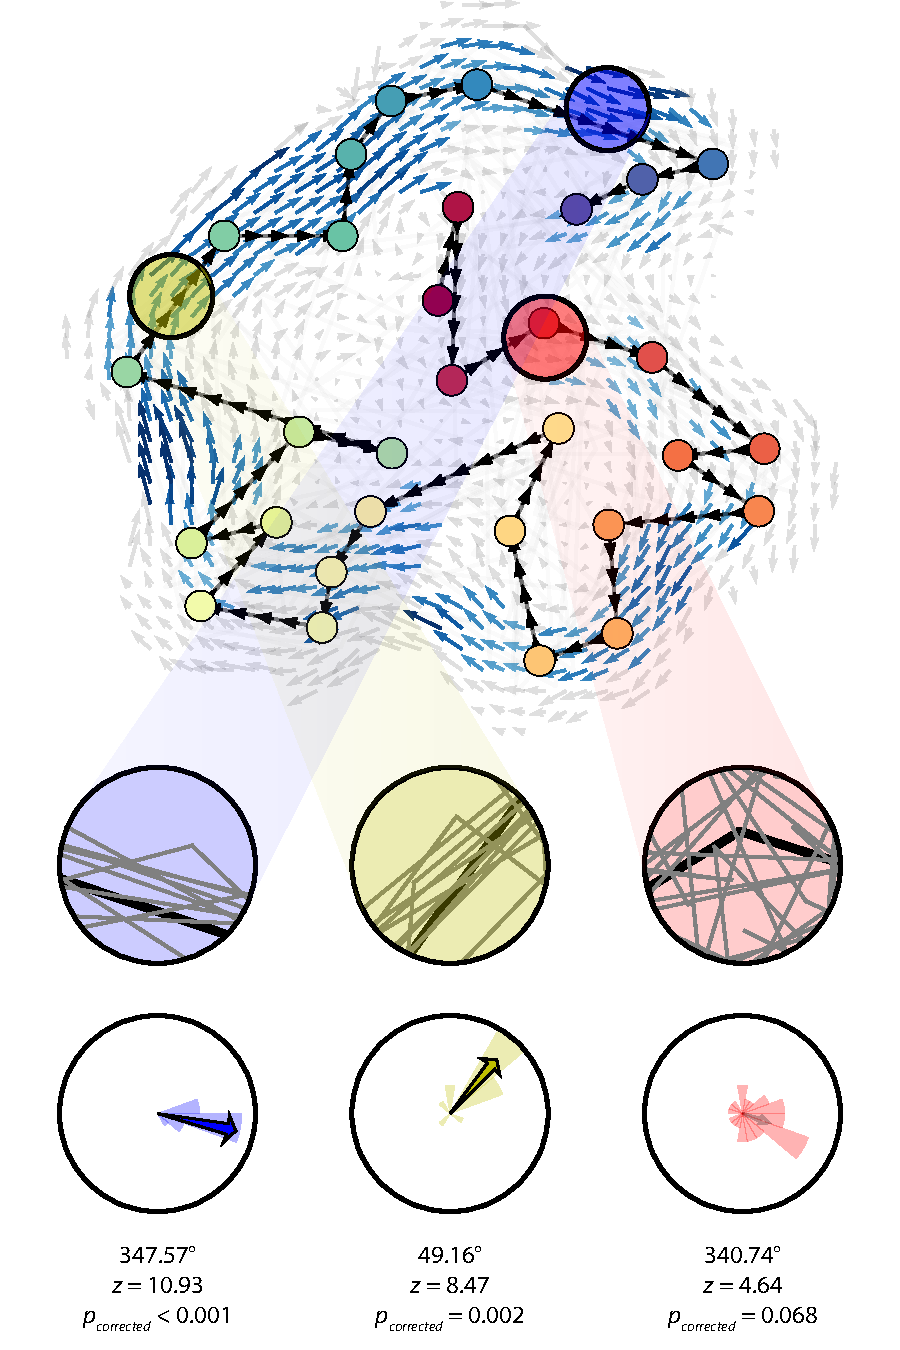
\includegraphics[width=0.6\textwidth]{figs/topic_space_flow}
\caption{\small \textbf{Methods detail for recall trajectory analysis displayed in Figure~\trajectories B} \textbf{A.} This panel replicates Figure~\trajectories B in the \textit{Main text}, but with two additions.  First, individual participants' recall trajectories are displayed (faintly) as light gray lines.  Second, three locations on the trajectory have been highlighted (blue, yellow, and red circles).  \textbf{B.}  These zoomed-in views of the locations highlighted in Panel A show the average trajectory (black) and individual participants' trajectories (gray lines) that intersect the given region of topic space.  \textbf{C.} For each circular region of topic space tiling the 2D embedding plane displayed in Panel A, we compute the distribution of angles formed between each participant's trajectory segment (i.e., the point at which the trajectory enters and exists the region of topic space) and the $x$-axis.  The distributions of angles for these three example regions are displayed in the colored rose plots.  We use Rayleigh tests to assign an arrow direction, length, and color for that region of topic space.  Arrows displayed in color are significant at the $p < 0.05$ level (corrected).  The arrow directions are oriented according to the circular means of each distribution, and the arrow lengths are proportional to the lengths of those mean vectors.  The example regions have been oriented from left to right in decreasing order of consistency across participants.}
\label{fig:arrows-methods}
\end{figure}
\FloatBarrier

\newpage
\subsection*{Participant-level figures referenced in the main text}
\vspace*{\fill}

\begin{figure}[p!]
\centering
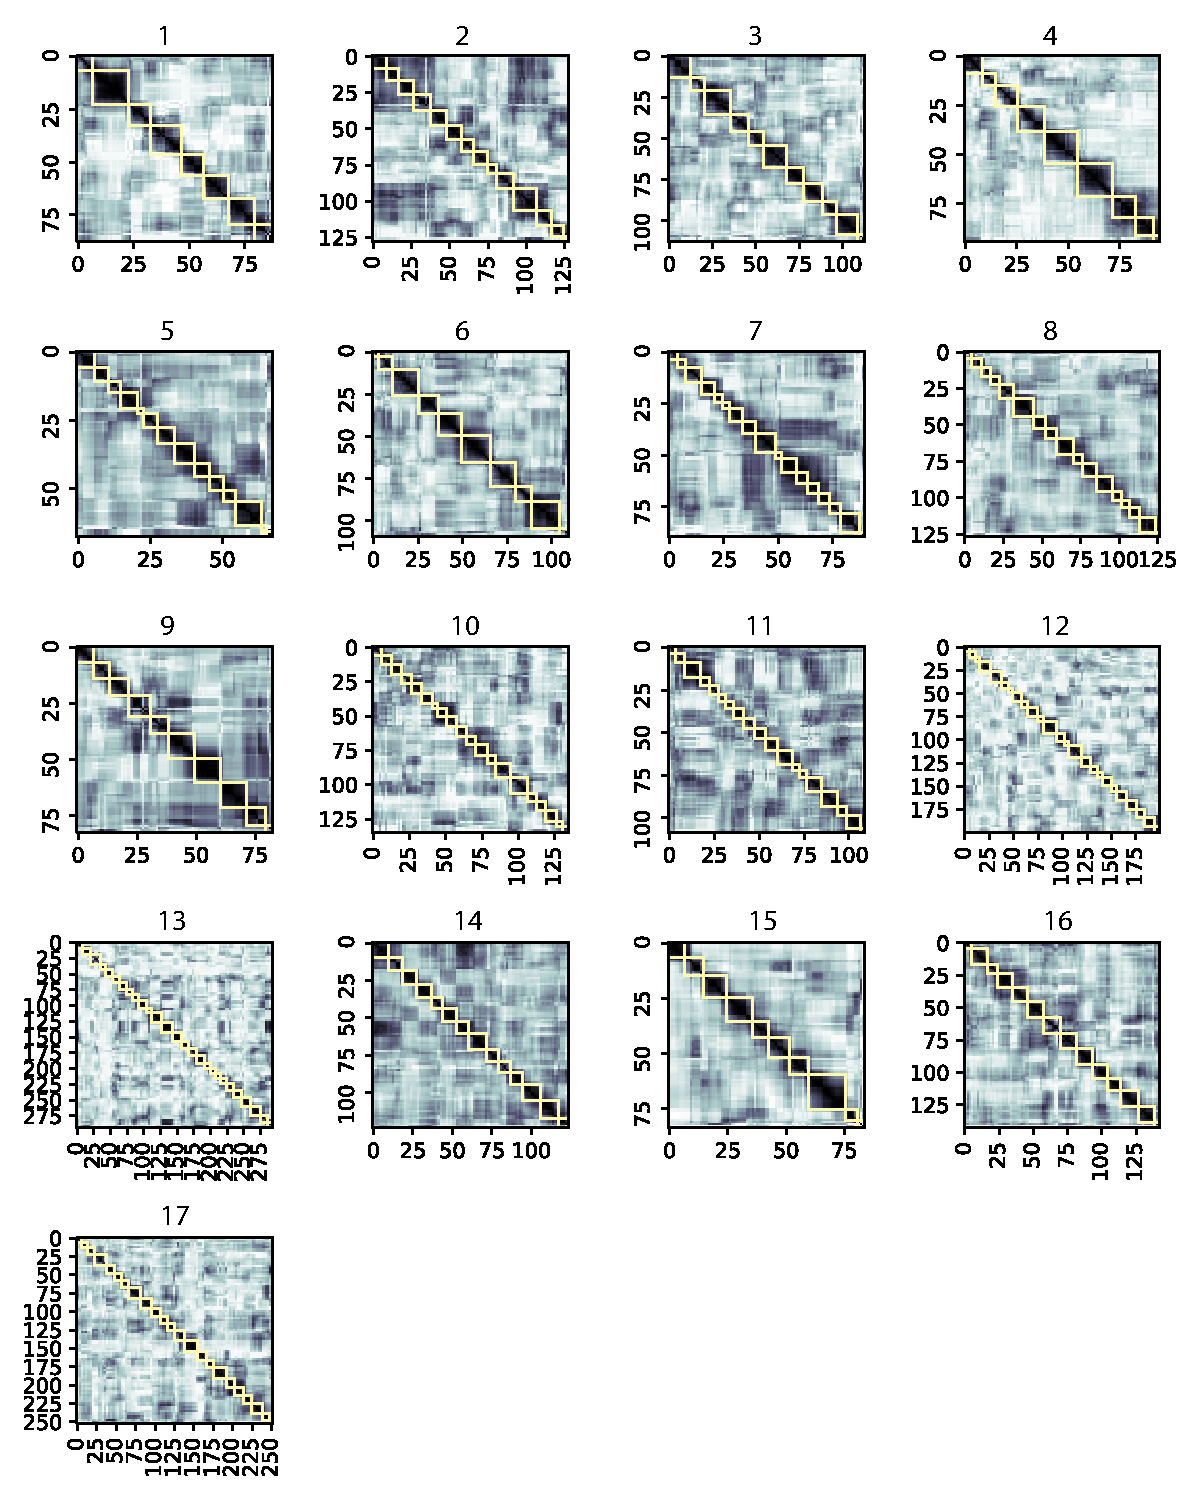
\includegraphics[width=\textwidth]{figs/corrmats}
\caption{\small \textbf{Recall temporal correlation matrices and event segmentation fits.} Each panel is in the same format as Figure~\topicprops E in the main text.  The yellow boxes indicate HMM-identified event boundaries.}
\label{fig:corrmats}
\end{figure}

\begin{figure}[p!]
\centering
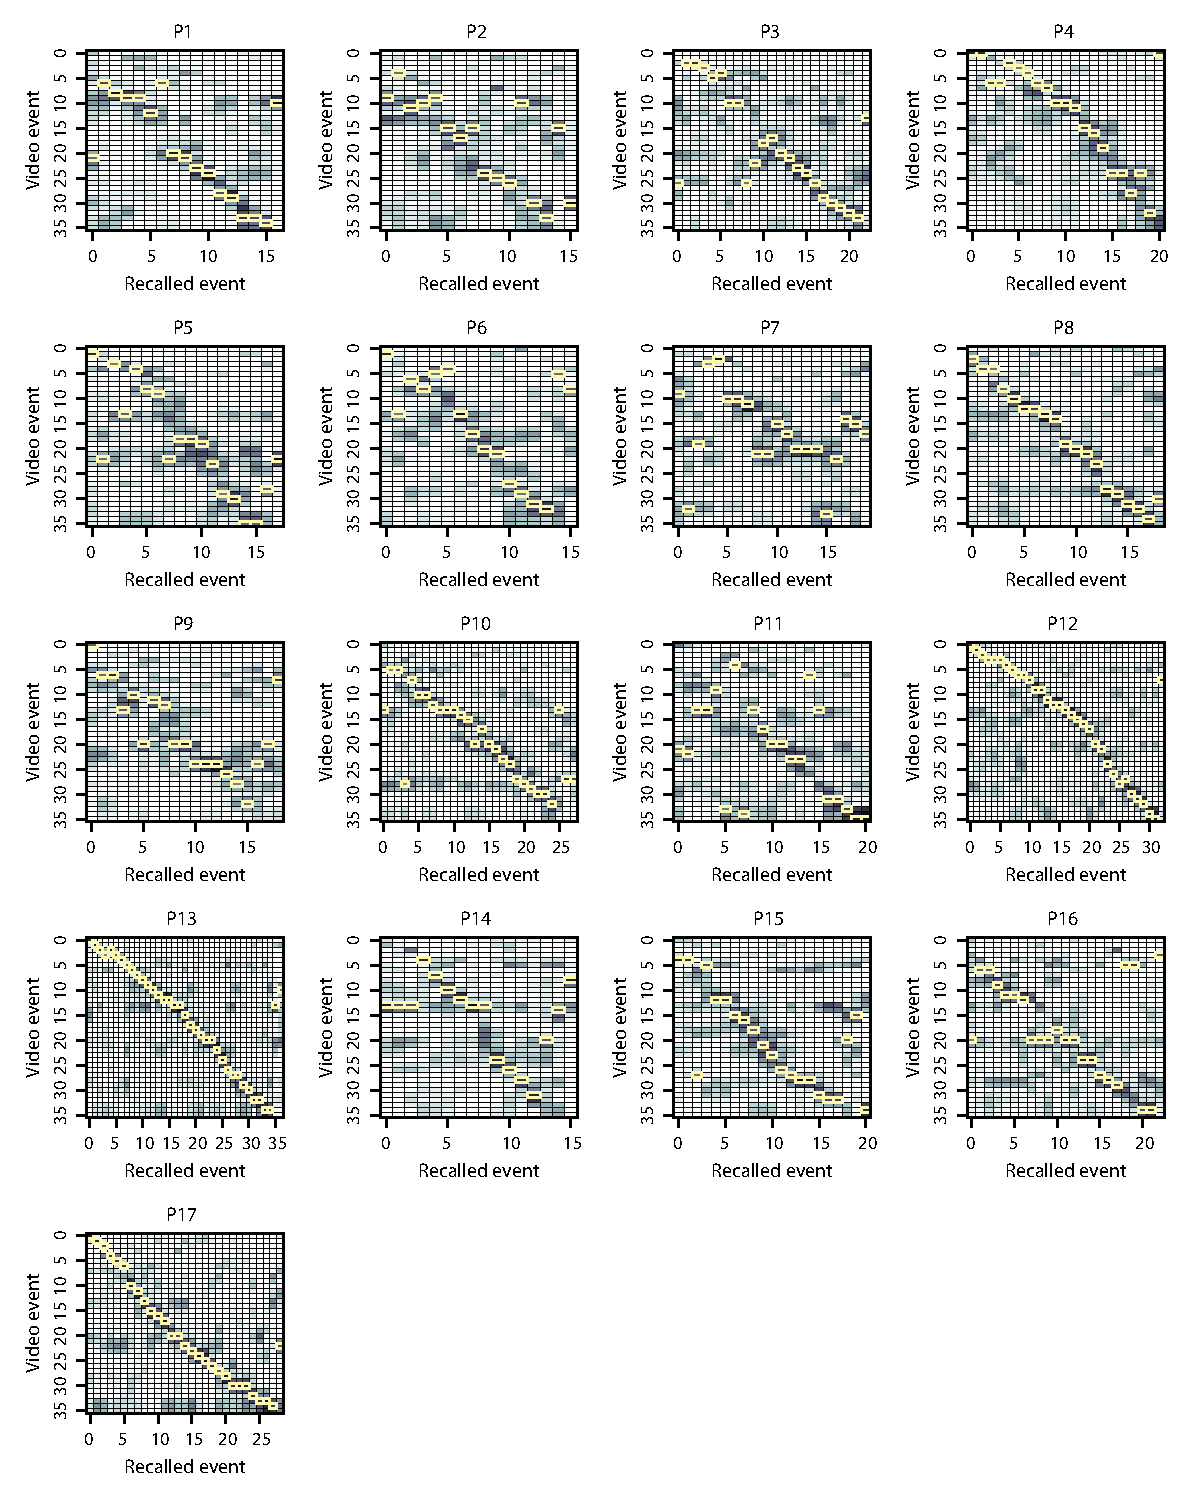
\includegraphics[width=\textwidth]{figs/matchmats}
\caption{\small \textbf{Episode-recall event correlation matrices.}  Each panel is in the same format as Figure~\topicprops G in the main text.  The yellow boxes mark the matched episode event for each recall event (i.e., the maximum correlation in each column).}
\label{fig:matchmats}
\end{figure}

\begin{figure}[p!]
\centering
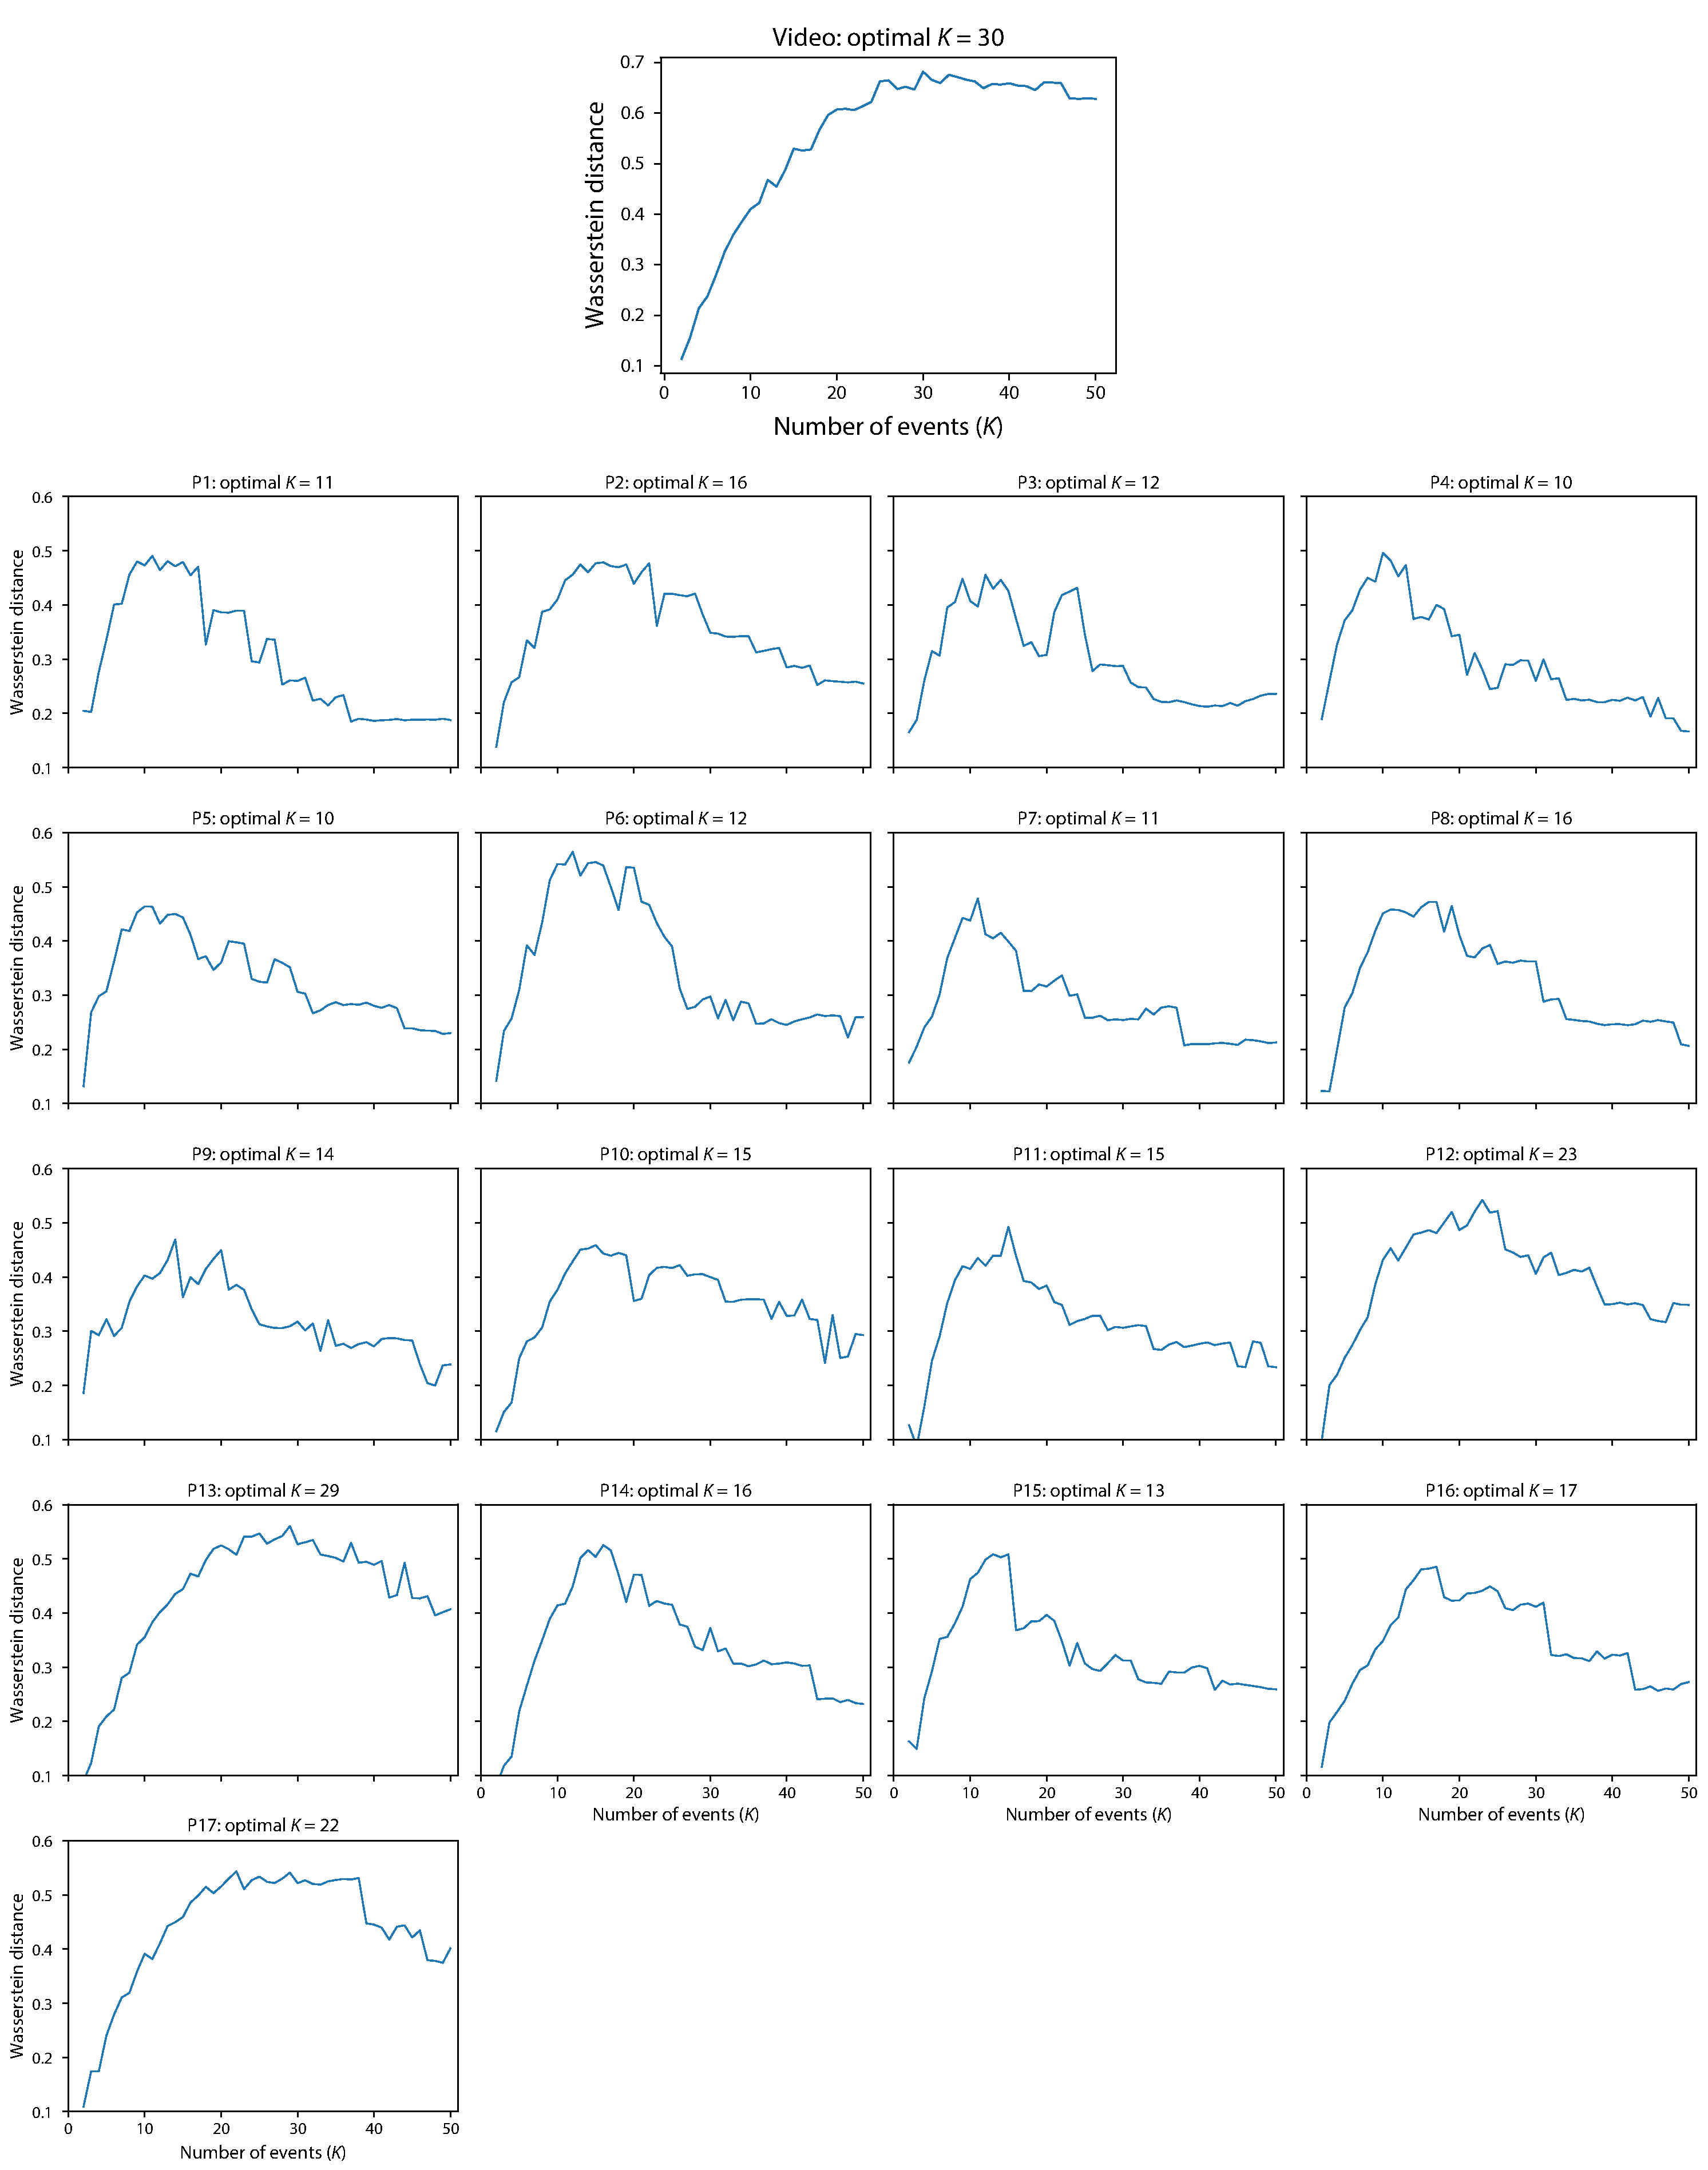
\includegraphics[width=.92\textwidth]{figs/k_optimization}
\caption{\small \textbf{Episode and recall topic proportions matrix \textit{K}-optimization functions.}  We selected the optimal $K$-value for the episode and each recall topic proportions matrix using the formula described in \textit{Methods}. This computation resulted in a curve for each matrix, describing the Wasserstein distance between the distributions of within-event and across-event topic vector correlations, as a function of $K$.}
\label{fig:k_optimization}
\end{figure}
\end{document}